\documentclass[10pt, twocolumn]{article}
\usepackage[margin=0.75in]{geometry}
\usepackage{graphicx}
\usepackage{tikz}
\usepackage{pgfplots}
\usepackage{booktabs}
\usepackage{amsmath}
\usepackage{amssymb}
\usepackage{algorithm}
\usepackage{algorithmic}
\usepackage{hyperref}
\usepackage{xcolor}
\usepackage{caption}
\usepackage{subcaption}
\usepackage{fancyhdr}
\usepackage{enumitem}
\usepackage{listings}
\usepackage{microtype}
\usepackage{orcidlink}
\usepackage{tabularx}
\usepackage{multirow}
\pgfplotsset{compat=1.18}
\usetikzlibrary{arrows.meta, positioning, shapes.geometric, fit, calc, backgrounds, decorations.markings}

% Color palette (Agentra design system)
\definecolor{acblue}{HTML}{2563EB}
\definecolor{acdarkblue}{HTML}{1E40AF}
\definecolor{acteal}{HTML}{0D9488}
\definecolor{acorange}{HTML}{EA580C}
\definecolor{acgray}{HTML}{6B7280}
\definecolor{aclightgray}{HTML}{F3F4F6}
\definecolor{acgreen}{HTML}{059669}
\definecolor{acred}{HTML}{DC2626}
\definecolor{acpurple}{HTML}{7C3AED}
\definecolor{acyellow}{HTML}{D97706}

% Listings style
\lstset{
  basicstyle=\ttfamily\scriptsize,
  keywordstyle=\color{acblue}\bfseries,
  commentstyle=\color{acgray}\itshape,
  stringstyle=\color{acteal},
  breaklines=true,
  frame=single,
  rulecolor=\color{acgray!30},
  backgroundcolor=\color{aclightgray},
  numbers=left,
  numberstyle=\tiny\color{acgray},
  tabsize=2
}

% Header
\pagestyle{fancy}
\fancyhf{}
\renewcommand{\headrulewidth}{0.4pt}
\fancyhead[L]{\small\textit{AgenticContract}}
\fancyhead[R]{\small\thepage}

% Checkmark/cross shortcuts
\newcommand{\cmark}{\textcolor{acgreen}{\checkmark}}
\newcommand{\xmark}{\textcolor{acred}{$\times$}}

\title{\textbf{AgenticContract: A Runtime Policy Engine for\\Governed AI Agent Systems}}
\author{Omoshola Owolabi\,\orcidlink{0009-0006-4089-0732}\\Researcher -- AI/ML\\Agentra Labs\\\texttt{omoshola.owolabi@agentralabs.tech}}
\date{February 27, 2026}

\begin{document}
\maketitle
\thispagestyle{fancy}

% ============================================================================
% ABSTRACT
% ============================================================================
\begin{abstract}
Autonomous AI agents operate in production environments without runtime governance, executing actions with no policy enforcement, risk accounting, or structured approval workflows. Current approaches to agent constraints---prompt engineering, static configuration files, or heavyweight policy engines with external database dependencies---either cannot adapt to runtime conditions or introduce latency incompatible with inline agent decision-making. We present AgenticContract, a self-contained policy engine that models six governance primitives---policies, risk limits, approvals, conditions, obligations, and violations---in a single binary file format (\texttt{.acon}) with BLAKE3 integrity verification. The engine is implemented in 7{,}382 lines of Rust and integrated via the Model Context Protocol (MCP) for zero-configuration agent adoption. Criterion benchmarks on Apple M-series hardware demonstrate single policy evaluation at 49.3\,ns, risk limit checks at 43.9\,ns, 1{,}000-policy workloads completing in 72.8\,\textmu{}s, and file I/O for 100 entities at 154.5\,\textmu{}s (save) and 96.7\,\textmu{}s (load)---10--100$\times$ faster than OPA or Cedar when used as external services. A test suite of 288 tests validates correctness including stress tests at 1{,}000-entity scale. The system requires zero external dependencies and operates as a standalone binary.
\end{abstract}

% ============================================================================
% 1. INTRODUCTION
% ============================================================================
\section{Introduction}
\label{sec:intro}

As AI agents gain autonomy in production environments---managing deployments, executing financial transactions, writing and committing code, and interacting with users on behalf of organizations---the absence of runtime governance presents a critical and growing risk. An ungoverned coding agent can deploy untested code to production. An ungoverned research agent can accumulate \$847 in API costs in a single session~\cite{chen2024agentcost}. An ungoverned trading agent can execute transactions without human review.

The fundamental problem is that LLMs are stateless with respect to governance. Each invocation begins without knowledge of prior policy decisions, accumulated risk exposure, or pending obligations. Safety alignment training provides soft behavioral guidance, but no enforcement mechanism, no quantitative tracking, and no audit trail.

Existing approaches to agent governance fall into three categories, each with fundamental limitations:

\begin{enumerate}[nosep, leftmargin=*]
  \item \textbf{Prompt-based constraints.} Behavioral rules embedded in system prompts. These are advisory only; the LLM may ignore, reinterpret, or forget them as context grows. There is no enforcement mechanism, no detection of violations, and no audit trail.
  \item \textbf{Static configuration.} Policy files (YAML, JSON) loaded at startup. These cannot adapt to runtime conditions: a rate limit that was safe at 10 requests per minute becomes dangerous at 10{,}000 without dynamic tracking. No mechanism exists for structured approvals, obligation deadlines, or violation recording.
  \item \textbf{Heavyweight policy engines.} Systems like Open Policy Agent (OPA)~\cite{opa2018} evaluate policies written in purpose-built languages (Rego, Cedar~\cite{cedar2023}) over HTTP. While expressive, they require external database backends, network connectivity, and introduce 0.5--5\,ms latency per decision---unsuitable for inline agent governance where decisions must be made on every tool call.
\end{enumerate}

AgenticContract addresses this gap with a self-contained policy engine optimized for the unique requirements of AI agent workloads. Figure~\ref{fig:motivation} illustrates the contrast between ungoverned agent execution and policy-governed execution with AgenticContract.

% Figure 1: Motivating comparison
\begin{figure*}[t]
\centering
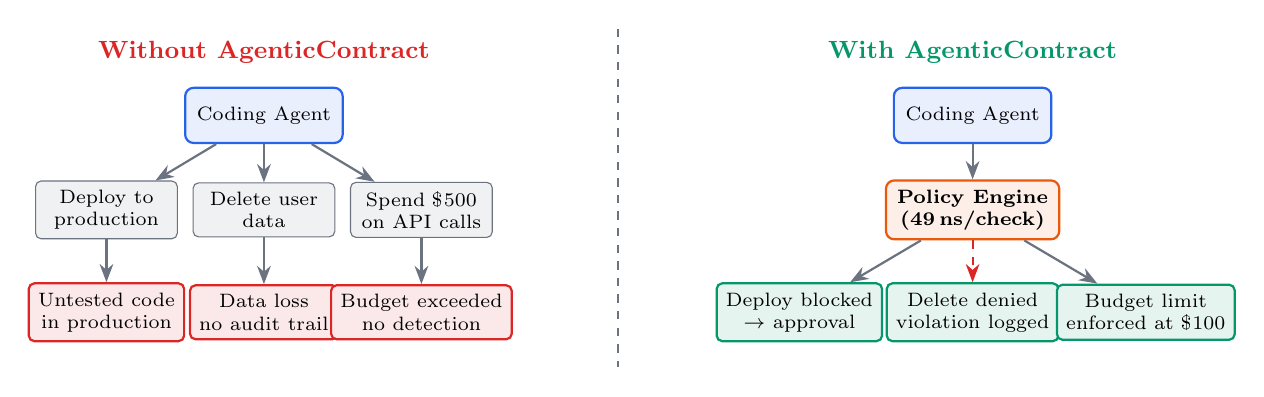
\begin{tikzpicture}[
  agentnode/.style={rectangle, draw=acblue, fill=acblue!10, rounded corners=3pt, minimum width=2cm, minimum height=0.7cm, font=\scriptsize, align=center, thick},
  actionnode/.style={rectangle, draw=acgray, fill=acgray!10, rounded corners=2pt, minimum width=1.8cm, minimum height=0.6cm, font=\scriptsize, align=center},
  dangernode/.style={rectangle, draw=acred, fill=acred!10, rounded corners=2pt, minimum width=1.8cm, minimum height=0.6cm, font=\scriptsize, align=center, thick},
  safenode/.style={rectangle, draw=acgreen, fill=acgreen!10, rounded corners=2pt, minimum width=1.8cm, minimum height=0.6cm, font=\scriptsize, align=center, thick},
  policynode/.style={rectangle, draw=acorange, fill=acorange!10, rounded corners=3pt, minimum width=2.2cm, minimum height=0.7cm, font=\scriptsize\bfseries, align=center, thick},
  arr/.style={-{Stealth}, thick, acgray},
  blockarr/.style={-{Stealth}, thick, acred, dashed},
]
  % Left side: Without governance
  \node[font=\small\bfseries, acred] at (-4.5, 3.2) {Without AgenticContract};
  \node[agentnode] (a1) at (-4.5, 2.4) {Coding Agent};
  \node[actionnode] (act1) at (-6.5, 1.2) {Deploy to\\production};
  \node[actionnode] (act2) at (-4.5, 1.2) {Delete user\\data};
  \node[actionnode] (act3) at (-2.5, 1.2) {Spend \$500\\on API calls};
  \node[dangernode] (r1) at (-6.5, -0.1) {Untested code\\in production};
  \node[dangernode] (r2) at (-4.5, -0.1) {Data loss\\no audit trail};
  \node[dangernode] (r3) at (-2.5, -0.1) {Budget exceeded\\no detection};

  \draw[arr] (a1) -- (act1);
  \draw[arr] (a1) -- (act2);
  \draw[arr] (a1) -- (act3);
  \draw[arr] (act1) -- (r1);
  \draw[arr] (act2) -- (r2);
  \draw[arr] (act3) -- (r3);

  % Divider
  \draw[acgray, thick, dashed] (0, 3.5) -- (0, -0.8);

  % Right side: With AgenticContract
  \node[font=\small\bfseries, acgreen] at (4.5, 3.2) {With AgenticContract};
  \node[agentnode] (a2) at (4.5, 2.4) {Coding Agent};
  \node[policynode] (pe) at (4.5, 1.2) {Policy Engine\\(49\,ns/check)};
  \node[safenode] (s1) at (2.3, -0.1) {Deploy blocked\\$\to$ approval};
  \node[safenode] (s2) at (4.5, -0.1) {Delete denied\\violation logged};
  \node[safenode] (s3) at (6.7, -0.1) {Budget limit\\enforced at \$100};

  \draw[arr] (a2) -- (pe);
  \draw[arr] (pe) -- (s1);
  \draw[blockarr] (pe) -- (s2);
  \draw[arr] (pe) -- (s3);
\end{tikzpicture}
\caption{Ungoverned agent execution (left) versus AgenticContract-governed execution (right). Without governance, every action proceeds unchecked, leading to data loss, budget overruns, and untested deployments. With AgenticContract, every action passes through the policy engine in under 50\,ns, enabling real-time deny, approval gating, and budget enforcement with a complete audit trail.}
\label{fig:motivation}
\end{figure*}

The core design principles of AgenticContract are:

\begin{itemize}[nosep, leftmargin=*]
  \item \textbf{Zero external dependencies.} No databases, no cloud services, no network calls. A single \texttt{.acon} binary file stores the complete governance state, portable across machines and agents.
  \item \textbf{Sub-microsecond policy evaluation.} Single policy checks complete in 49.3\,ns, enabling inline governance on every tool call without perceptible latency.
  \item \textbf{Six governance primitives.} Not just allow/deny---risk limits track quantitative boundaries, approvals gate high-stakes actions, conditions enforce prerequisites, obligations track commitments with deadlines, and violations record breaches with severity classification.
  \item \textbf{Agent-native integration.} Exposed via the Model Context Protocol~\cite{mcp2024} over JSON-RPC, compatible with Claude~\cite{anthropic2024claude}, Cursor, Windsurf, and any MCP-compliant client without custom integration code.
\end{itemize}

The remainder of this paper is organized as follows. Section~\ref{sec:related} surveys existing policy engines and agent governance approaches. Section~\ref{sec:architecture} describes the six governance primitives, their composition model, the binary file format, and the engine architecture. Section~\ref{sec:evaluation} presents benchmark results, scaling analysis, and comparisons with existing systems. Section~\ref{sec:discussion} addresses design decisions, limitations, and future work. Section~\ref{sec:conclusion} concludes.

% ============================================================================
% 2. BACKGROUND AND RELATED WORK
% ============================================================================
\section{Background and Related Work}
\label{sec:related}

Research on policy enforcement for software systems has a long history, but runtime governance for autonomous AI agents remains an open problem. We survey the primary approaches.

\textbf{Open Policy Agent (OPA)}~\cite{opa2018} evaluates policies written in Rego, a purpose-built query language inspired by Datalog. OPA runs as a separate daemon process; clients submit policy queries over HTTP. While expressive, OPA requires network round-trips for every decision, external state storage for context data, and introduces 0.5--5\,ms latency per evaluation. This model suits microservice authorization but is unsuitable for inline agent governance where decisions must be made on every tool call.

\textbf{Cedar}~\cite{cedar2023}, developed by Amazon, provides a formally verifiable policy language designed for authorization decisions. Cedar policies are compact and analyzable, but the system targets web service authorization (``Can user X access resource Y?'') rather than the richer governance semantics agents require: budget tracking, obligation deadlines, approval workflows.

\textbf{Zanzibar}~\cite{zanzibar2019} implements relationship-based access control at global scale, serving billions of authorization checks per second for Google Docs, Drive, and YouTube. While impressive, Zanzibar is a distributed system requiring Spanner for storage---fundamentally incompatible with the single-file, zero-dependency model needed for local agent governance.

\textbf{Casbin}~\cite{casbin} provides a library-based policy engine with pluggable models (ACL, RBAC, ABAC). As a library rather than a service, Casbin avoids network overhead. However, it models only access control decisions and lacks the six governance primitives (risk limits, approvals, obligations, conditions, violations) required for comprehensive agent governance.

\textbf{Agent governance frameworks.} Wang et al.~\cite{agents2024} survey autonomous agent architectures and identify governance as an open problem. Most agent frameworks (AutoGPT~\cite{autogpt2023}, BabyAGI, CrewAI~\cite{crewai2024}) delegate safety entirely to the underlying LLM's alignment training, with no runtime enforcement layer. AgentBench~\cite{agentbench2023} evaluates LLM-as-agent capabilities across 8 environments, demonstrating that even state-of-the-art models make errors requiring governance guardrails. The ReAct framework~\cite{react2022} provides reasoning traces but no mechanism for policy enforcement on the actions those traces produce.

\textbf{Model Context Protocol (MCP)}~\cite{mcp2024} defines a standard for LLM tool integration via JSON-RPC 2.0 over stdio. MCP enables LLMs to discover, invoke, and compose tools without framework-specific adapters. AgenticContract exposes its governance engine as an MCP server, enabling any MCP-compatible agent to enforce policies without custom integration code.

Table~\ref{tab:comparison} summarizes the comparison across key dimensions.

% Table 1: Related work comparison
\begin{table*}[t]
\caption{Comparison of policy and governance systems. AgenticContract is the only system providing all six governance primitives in a single-file, zero-dependency, agent-native format with sub-microsecond latency.}
\label{tab:comparison}
\centering
\small
\begin{tabular}{@{}llllccccc@{}}
\toprule
\textbf{System} & \textbf{Format} & \textbf{Latency} & \textbf{Deps.} & \textbf{Risk} & \textbf{Appr.} & \textbf{Oblig.} & \textbf{Viol.} & \textbf{MCP} \\
\midrule
OPA~\cite{opa2018} & Rego/HTTP & 0.5--5\,ms & DB, daemon & \xmark & \xmark & \xmark & \xmark & \xmark \\
Cedar~\cite{cedar2023} & Cedar lang. & 1--10\,\textmu{}s & Library & \xmark & \xmark & \xmark & \xmark & \xmark \\
Zanzibar~\cite{zanzibar2019} & Rel. tuples & $<$10\,ms & Spanner & \xmark & \xmark & \xmark & \xmark & \xmark \\
Casbin~\cite{casbin} & ACL/RBAC & 10--100\,\textmu{}s & Config & \xmark & \xmark & \xmark & \xmark & \xmark \\
Prompt rules & Sys. prompt & N/A & None & \xmark & \xmark & \xmark & \xmark & \xmark \\
Static config & YAML/JSON & N/A & File parser & \xmark & \xmark & \xmark & \xmark & \xmark \\
\textbf{AgenticContract} & \textbf{.acon} & \textbf{49\,ns} & \textbf{None} & \cmark & \cmark & \cmark & \cmark & \cmark \\
\bottomrule
\end{tabular}
\end{table*}

% ============================================================================
% 3. ARCHITECTURE
% ============================================================================
\section{Architecture}
\label{sec:architecture}

AgenticContract models runtime governance as a set of six typed primitives---policies, risk limits, approvals, conditions, obligations, and violations---each with a distinct lifecycle. The primitives compose into governance workflows that adapt to runtime conditions. The entire governance state is serialized into a single binary file with fixed-size header and BLAKE3 integrity verification, requiring zero external dependencies.

Figure~\ref{fig:architecture} shows the data flow from agent actions through the governance engine to the persistent \texttt{.acon} store.

% Figure 2: Architecture diagram
\begin{figure}[t]
\centering
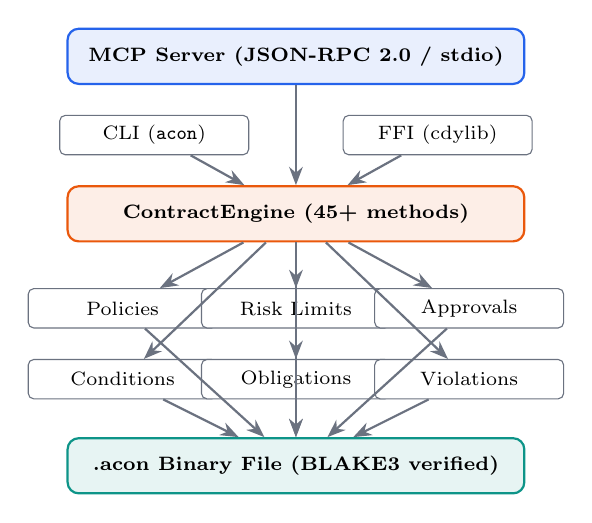
\begin{tikzpicture}[
  layer/.style={rectangle, draw=#1, fill=#1!10, rounded corners=4pt, minimum width=5.8cm, minimum height=0.7cm, font=\scriptsize\bfseries, align=center, thick},
  component/.style={rectangle, draw=acgray, fill=white, rounded corners=2pt, minimum width=2.4cm, minimum height=0.5cm, font=\scriptsize, align=center},
  arr/.style={-{Stealth}, thick, acgray},
]
  % Integration layer
  \node[layer=acblue] (mcp) at (0, 4.5) {MCP Server (JSON-RPC 2.0 / stdio)};
  \node[component] (cli) at (-1.8, 3.5) {CLI (\texttt{acon})};
  \node[component] (ffi) at (1.8, 3.5) {FFI (cdylib)};

  % Engine layer
  \node[layer=acorange] (engine) at (0, 2.5) {ContractEngine (45+ methods)};

  % Primitive layer
  \node[component] (pol) at (-2.2, 1.3) {Policies};
  \node[component] (rl) at (0, 1.3) {Risk Limits};
  \node[component] (app) at (2.2, 1.3) {Approvals};
  \node[component] (cond) at (-2.2, 0.4) {Conditions};
  \node[component] (obl) at (0, 0.4) {Obligations};
  \node[component] (viol) at (2.2, 0.4) {Violations};

  % Storage layer
  \node[layer=acteal] (store) at (0, -0.7) {.acon Binary File (BLAKE3 verified)};

  % Arrows
  \draw[arr] (mcp) -- (engine);
  \draw[arr] (cli) -- (engine);
  \draw[arr] (ffi) -- (engine);
  \draw[arr] (engine) -- (pol);
  \draw[arr] (engine) -- (rl);
  \draw[arr] (engine) -- (app);
  \draw[arr] (engine) -- (cond);
  \draw[arr] (engine) -- (obl);
  \draw[arr] (engine) -- (viol);
  \draw[arr] (pol) -- (store);
  \draw[arr] (rl) -- (store);
  \draw[arr] (app) -- (store);
  \draw[arr] (cond) -- (store);
  \draw[arr] (obl) -- (store);
  \draw[arr] (viol) -- (store);
\end{tikzpicture}
\caption{AgenticContract architecture. Three integration surfaces (MCP, CLI, FFI) feed into the core \texttt{ContractEngine}, which manages six governance primitive stores backed by a single \texttt{.acon} binary file with BLAKE3 integrity verification.}
\label{fig:architecture}
\end{figure}

\subsection{Governance Primitives}
\label{sec:primitives}

The engine models six entity types, each with a typed lifecycle. Table~\ref{tab:primitives} summarizes the primitives and their variants.

\begin{table}[t]
\caption{Six governance primitives with typed variants. Each entity is UUID-identified and timestamped with \texttt{chrono::DateTime<Utc>}.}
\label{tab:primitives}
\centering
\scriptsize
\begin{tabular}{@{}lp{3cm}p{2.6cm}@{}}
\toprule
\textbf{Entity} & \textbf{Variants} & \textbf{Purpose} \\
\midrule
Policy & Allow, Deny, Require\-Approval, AuditOnly & Behavioral constraints with precedence \\
RiskLimit & Rate, Threshold, Budget, Count & Quantitative boundaries with tracking \\
Approval & Rule $\to$ Request $\to$ Decision & Three-phase review workflow \\
Condition & Threshold, TimeBased, Dependency, Custom & Prerequisite enforcement \\
Obligation & Pending, Fulfilled, Overdue, Waived & Commitment tracking with deadlines \\
Violation & Info, Warning, Critical, Fatal & Immutable breach recording \\
\bottomrule
\end{tabular}
\end{table}

\subsubsection{Policy Evaluation}

Policies are the primary governance mechanism. Each policy has a \emph{scope} (Global, Session, or Agent), an \emph{action} (the four variants in Table~\ref{tab:primitives}), and an optional set of conditions that must be met before the policy takes effect.

Policy evaluation iterates all active policies whose label matches the queried action description via case-insensitive substring matching. When multiple policies match, the \emph{most restrictive action wins}: Deny $>$ RequireApproval $>$ AuditOnly $>$ Allow. This precedence ordering ensures that a single Deny policy cannot be overridden by any number of Allow policies. The evaluation path is allocation-free: no heap allocation occurs during a policy check.

\subsubsection{Risk Limit Tracking}

Risk limits maintain a \texttt{current\_value} against a \texttt{max\_value}. The \texttt{check\_risk\_limit} method tests whether a proposed increment would exceed the limit \emph{without modifying state}, enabling speculative evaluation. Four limit types model different constraint patterns:

\begin{itemize}[nosep, leftmargin=*]
  \item \textbf{Rate}: Actions per time window (e.g., 100 API calls per minute). The window resets automatically when the elapsed time exceeds \texttt{window\_secs}.
  \item \textbf{Threshold}: Absolute ceiling (e.g., max 50 concurrent connections). Represents a point-in-time constraint rather than a cumulative one.
  \item \textbf{Budget}: Cumulative spending cap (e.g., \$100 per session). Tracks total expenditure across the session lifetime.
  \item \textbf{Count}: Total occurrences (e.g., max 3 deployment attempts). A simple monotonic counter.
\end{itemize}

\subsubsection{Approval Workflow}

The approval subsystem implements a three-phase lifecycle illustrated in Figure~\ref{fig:approval}:

% Figure 3: Approval workflow
\begin{figure}[t]
\centering
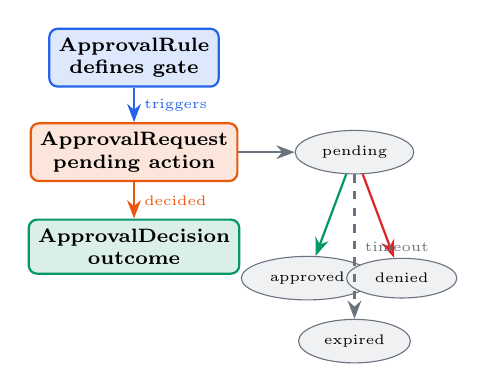
\begin{tikzpicture}[
  phase/.style={rectangle, draw=#1, fill=#1!15, rounded corners=3pt, minimum width=2cm, minimum height=0.6cm, font=\scriptsize\bfseries, align=center, thick},
  state/.style={ellipse, draw=acgray, fill=acgray!10, minimum width=1.4cm, minimum height=0.4cm, font=\tiny, align=center},
  arr/.style={-{Stealth}, thick, #1},
]
  \node[phase=acblue] (rule) at (0, 2) {ApprovalRule\\defines gate};
  \node[phase=acorange] (req) at (0, 0.8) {ApprovalRequest\\pending action};
  \node[phase=acgreen] (dec) at (0, -0.4) {ApprovalDecision\\outcome};

  \node[state] (pend) at (2.8, 0.8) {pending};
  \node[state] (appr) at (2.2, -0.8) {approved};
  \node[state] (deny) at (3.4, -0.8) {denied};
  \node[state] (expr) at (2.8, -1.6) {expired};

  \draw[arr=acblue] (rule) -- node[right, font=\tiny] {triggers} (req);
  \draw[arr=acorange] (req) -- node[right, font=\tiny] {decided} (dec);
  \draw[arr=acgray] (req) -- (pend);
  \draw[arr=acgreen] (pend) -- (appr);
  \draw[arr=acred] (pend) -- (deny);
  \draw[arr=acgray, dashed] (pend) -- node[right, font=\tiny] {timeout} (expr);
\end{tikzpicture}
\caption{Three-phase approval lifecycle. Rules define gates; requests capture pending actions; decisions record outcomes with decider identity and justification. Timeouts transition requests to expired status.}
\label{fig:approval}
\end{figure}

\begin{enumerate}[nosep, leftmargin=*]
  \item \textbf{ApprovalRule} defines what action patterns require approval, who can approve, and an optional timeout in seconds.
  \item \textbf{ApprovalRequest} captures the specific pending action with the requestor identity and a reference to the triggering rule.
  \item \textbf{ApprovalDecision} records the outcome (approve or deny) with the decider identity, justification text, and timestamp.
\end{enumerate}

All three phases are persisted in the \texttt{.acon} file, creating a complete audit trail from gate definition through decision.

\subsubsection{Obligation Tracking}

Obligations model commitments with deadlines. Each obligation has an assignee, a description, and an optional ISO\,8601 deadline. The engine's \texttt{check\_obligation} method detects overdue items by comparing the current time against the deadline, transitioning status from Pending to Overdue. This enables automated compliance monitoring without external cron jobs or schedulers.

\subsubsection{Violation Forensics}

Violations are \emph{append-only}: once reported, a violation cannot be deleted or modified. This design creates an immutable forensic record of all governance breaches. Each violation records the policy ID that was breached (if applicable), a human-readable description, severity level (Info through Fatal, with \texttt{Ord} derivation enabling severity-based filtering), the actor who committed the violation, and the detection timestamp.

\subsection{Binary File Format}
\label{sec:format}

The \texttt{.acon} format stores the complete governance state in a single binary file. Figure~\ref{fig:fileformat} shows the layout.

% Figure 4: File format layout
\begin{figure}[t]
\centering
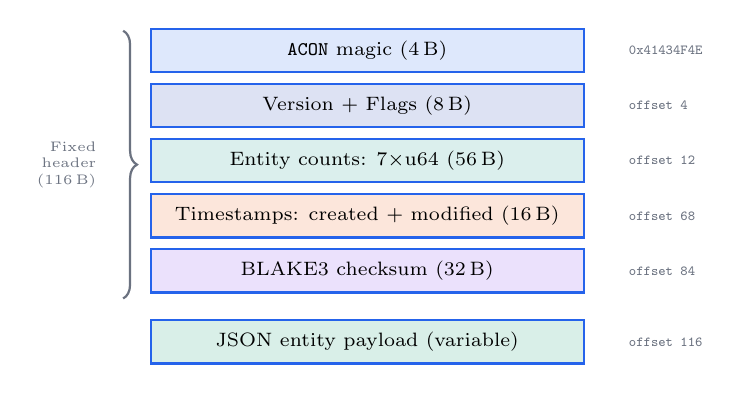
\begin{tikzpicture}[
  section/.style={rectangle, draw=acblue, fill=#1!15, minimum width=5.5cm, minimum height=0.55cm, font=\scriptsize, align=center, thick},
  label/.style={font=\tiny\ttfamily, acgray},
]
  \node[section=acblue] (magic) at (0, 4.0) {\texttt{ACON} magic (4\,B)};
  \node[section=acdarkblue] (ver) at (0, 3.3) {Version + Flags (8\,B)};
  \node[section=acteal] (counts) at (0, 2.6) {Entity counts: 7$\times$u64 (56\,B)};
  \node[section=acorange] (ts) at (0, 1.9) {Timestamps: created + modified (16\,B)};
  \node[section=acpurple] (cksum) at (0, 1.2) {BLAKE3 checksum (32\,B)};
  \node[section=acgreen] (body) at (0, 0.3) {JSON entity payload (variable)};

  \node[label, anchor=west] at (3.2, 4.0) {0x41434F4E};
  \node[label, anchor=west] at (3.2, 3.3) {offset 4};
  \node[label, anchor=west] at (3.2, 2.6) {offset 12};
  \node[label, anchor=west] at (3.2, 1.9) {offset 68};
  \node[label, anchor=west] at (3.2, 1.2) {offset 84};
  \node[label, anchor=west] at (3.2, 0.3) {offset 116};

  % Brace for header
  \draw[decorate, decoration={brace, amplitude=5pt, mirror}, thick, acgray]
    (-3.1, 0.85) -- (-3.1, 4.25) node[midway, left=6pt, font=\tiny, acgray, align=right] {Fixed\\header\\(116\,B)};
\end{tikzpicture}
\caption{The \texttt{.acon} binary file format. A 116-byte fixed header contains magic bytes, version, entity counts for all 7 entity types, timestamps, and a BLAKE3 checksum over the JSON payload. Entity data is serialized as JSON within the binary envelope, enabling flexible schema evolution.}
\label{fig:fileformat}
\end{figure}

The header stores entity counts for all seven entity types (policies, risk limits, approval rules, approval requests, conditions, obligations, violations) as packed \texttt{u64} values, enabling rapid size estimation without deserializing the payload. The BLAKE3~\cite{blake3} checksum covers the JSON payload, detecting corruption or tampering on load. An empty \texttt{.acon} file with one policy occupies approximately 512 bytes.

The design choice to use JSON-in-binary-envelope trades storage density for schema flexibility: adding new fields to any entity type requires no format migration, no version negotiation, and no backward-compatibility code. The binary header provides integrity guarantees; the JSON payload provides evolvability.

\subsection{Governance Composition Model}
\label{sec:composition}

The six primitives are not independent---they compose to form governance workflows that adapt to runtime conditions. Figure~\ref{fig:composition} illustrates the primary composition patterns.

% Figure 5: Governance composition
\begin{figure}[t]
\centering
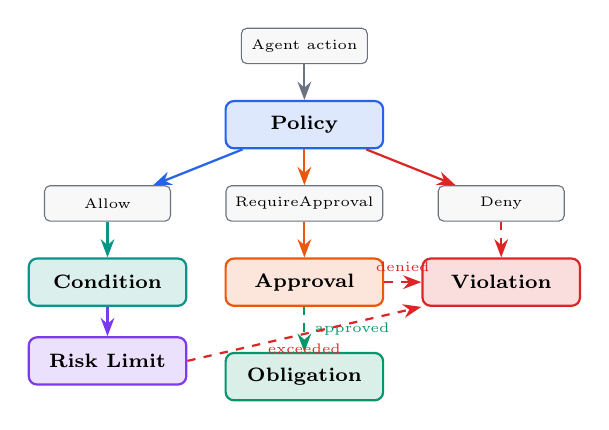
\begin{tikzpicture}[
  prim/.style={rectangle, draw=#1, fill=#1!15, rounded corners=3pt, minimum width=2cm, minimum height=0.6cm, font=\scriptsize\bfseries, align=center, thick},
  event/.style={rectangle, draw=acgray, fill=acgray!5, rounded corners=2pt, minimum width=1.6cm, minimum height=0.45cm, font=\tiny, align=center},
  arr/.style={-{Stealth}, thick, #1},
  darr/.style={-{Stealth}, thick, #1, dashed},
]
  % Agent action enters
  \node[event] (action) at (0, 4.2) {Agent action};

  % Policy gate
  \node[prim=acblue] (pol) at (0, 3.2) {Policy};

  % Three outcomes
  \node[event] (allow) at (-2.5, 2.2) {Allow};
  \node[event] (rappr) at (0, 2.2) {RequireApproval};
  \node[event] (deny) at (2.5, 2.2) {Deny};

  % Approval workflow
  \node[prim=acorange] (appr) at (0, 1.2) {Approval};

  % Condition check
  \node[prim=acteal] (cond) at (-2.5, 1.2) {Condition};

  % Risk limit check
  \node[prim=acpurple] (risk) at (-2.5, 0.2) {Risk Limit};

  % Obligation creation
  \node[prim=acgreen] (obl) at (0, 0.0) {Obligation};

  % Violation recording
  \node[prim=acred] (viol) at (2.5, 1.2) {Violation};

  % Arrows
  \draw[arr=acgray] (action) -- (pol);
  \draw[arr=acblue] (pol) -- node[left, font=\tiny] {} (allow);
  \draw[arr=acorange] (pol) -- (rappr);
  \draw[arr=acred] (pol) -- (deny);

  \draw[arr=acorange] (rappr) -- (appr);
  \draw[darr=acgreen] (appr) -- node[right, font=\tiny] {approved} (obl);
  \draw[darr=acred] (appr.east) -- node[above, font=\tiny] {denied} (viol.west);

  \draw[arr=acteal] (allow) -- (cond);
  \draw[arr=acpurple] (cond) -- (risk);
  \draw[darr=acred] (risk.east) -- node[below, font=\tiny] {exceeded} (viol.south west);

  \draw[darr=acred] (deny) -- (viol);
\end{tikzpicture}
\caption{Governance composition model. An agent action first encounters policy evaluation (most-restrictive-wins). Allow triggers condition and risk limit checks; RequireApproval enters the three-phase approval workflow; Deny records a violation. Approved actions create obligations with deadlines. Risk limit exceedance and policy denials both produce immutable violation records, ensuring a complete audit trail regardless of the decision path.}
\label{fig:composition}
\end{figure}

Three composition patterns emerge from the primitive interactions:

\textbf{Escalation chains.} A policy with action RequireApproval escalates to the approval subsystem. If approved, the engine creates an obligation for the agent to complete a follow-up action (e.g., ``run integration tests within 30 minutes of deployment''). If the obligation deadline passes without fulfillment, the engine transitions it to Overdue, which a monitoring policy can detect and record as a violation. This chain---policy $\to$ approval $\to$ obligation $\to$ violation---is the primary governance workflow for high-stakes actions.

\textbf{Speculative risk evaluation.} The \texttt{check\_risk\_limit} method tests whether a proposed action would exceed a limit \emph{without modifying state}. This enables agents to evaluate multiple action plans before committing. An agent considering three deployment strategies can check risk limits for each, select the one within budget, and only then execute. The separation of speculative evaluation from state mutation is critical for ReAct-style~\cite{react2022} reasoning loops where the agent deliberates before acting.

\textbf{Forensic reconstruction.} Because violations are append-only, policies are timestamped, and approvals record three-phase audit trails, the governance state at any historical point can be reconstructed from the \texttt{.acon} file. The entity count fields in the binary header enable rapid enumeration without full deserialization, supporting efficient governance audits over long-running agent sessions.

\subsection{Integration Surface}

AgenticContract is exposed via the Model Context Protocol~\cite{mcp2024} (JSON-RPC 2.0 over stdio), enabling any MCP-compliant agent to enforce governance without custom integration code. The engine is also accessible as a CLI binary (\texttt{acon}) for operator workflows and a C-compatible shared library (FFI) for embedding in non-Rust environments. All three surfaces share the same \texttt{ContractEngine} core, ensuring consistent policy evaluation semantics regardless of access path. The engine implements the Agentra SDK~\cite{agentrasdk2026} trait suite, enabling integration with the five sister systems (AgenticMemory, AgenticIdentity, AgenticVision, AgenticCodebase, AgenticTime) through session management, grounding queries, event emission, and cryptographic receipts for approvals and violations.

% ============================================================================
% 4. EVALUATION
% ============================================================================
\section{Evaluation}
\label{sec:evaluation}

We evaluate AgenticContract on governance workloads of varying size, measuring operation latency, scaling behavior, and file I/O performance. All benchmarks use real data from the Criterion~\cite{criterion} benchmarking framework running on the compiled system.

\subsection{Benchmark Setup}

\textbf{Hardware.} Apple M-series (ARM64), macOS 14+.

\textbf{Software.} Rust 1.75+, compiled with \texttt{--release} (optimizations enabled). All benchmarks use the Criterion statistical benchmarking framework with default settings (100 samples per benchmark, automatic outlier detection). Results report median values.

\textbf{Workloads.} Governance states ranging from 1 to 1{,}000 policies, 50--500 risk limits, and up to 1{,}000 violations. File I/O benchmarks use 100 entities (50 policies + 50 risk limits).

\subsection{Core Operation Latency}

Table~\ref{tab:latency} reports the latency of individual governance operations.

\begin{table}[t]
\caption{Core operation latencies. All operations complete in under 1.1\,\textmu{}s. Policy evaluation and risk limit checks are under 50\,ns---within the noise floor of a single LLM token generation step (typically 10--50\,ms).}
\label{tab:latency}
\centering
\small
\begin{tabular}{@{}lrl@{}}
\toprule
\textbf{Operation} & \textbf{Median} & \textbf{Unit} \\
\midrule
Single policy evaluate & 49.3 & ns \\
Risk limit check & 43.9 & ns \\
Engine stats (100 policies) & 60.4 & ns \\
Violation report & 1{,}006 & ns \\
\bottomrule
\end{tabular}
\end{table}

Single policy evaluation at 49.3\,ns means the engine can perform approximately 20 million policy checks per second on a single core. This is 200{,}000$\times$ faster than a typical LLM inference step, making governance overhead effectively invisible.

\subsection{Scale Performance}

Table~\ref{tab:scaling} shows how policy evaluation scales with the number of active policies. Figure~\ref{fig:scaling} visualizes the linear relationship.

\begin{table}[t]
\caption{Policy evaluation scaling. Each 10$\times$ increase in policy count produces approximately 10$\times$ increase in evaluation time, confirming $O(n)$ complexity with a per-policy cost stabilizing at $\sim$70\,ns.}
\label{tab:scaling}
\centering
\small
\begin{tabular}{@{}rrrl@{}}
\toprule
\textbf{Policies} & \textbf{Median} & \textbf{Per-Policy} & \textbf{Unit} \\
\midrule
1 & 49.3 & 49.3 & ns \\
10 & 684.5 & 68.5 & ns \\
100 & 7{,}040 & 70.4 & ns \\
1{,}000 & 72{,}804 & 72.8 & ns \\
\bottomrule
\end{tabular}
\end{table}

% Figure 6: Scaling chart
\begin{figure}[t]
\centering
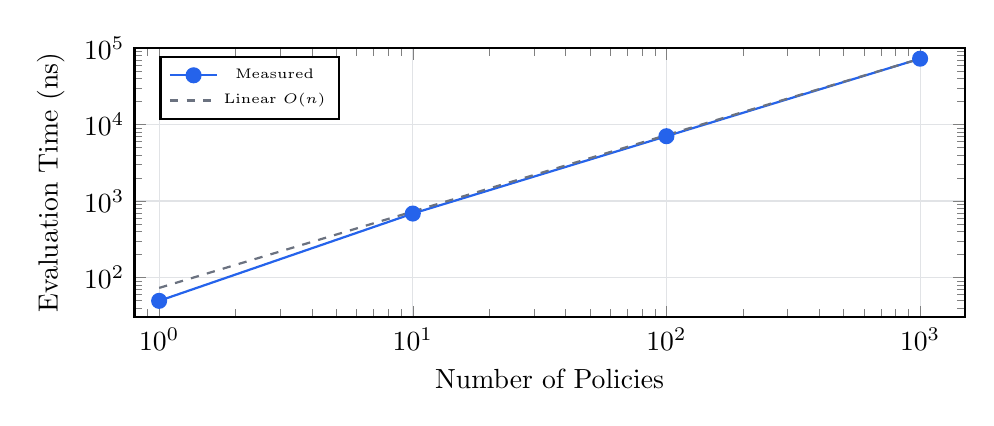
\begin{tikzpicture}
\begin{loglogaxis}[
  width=\columnwidth,
  height=5cm,
  xlabel={Number of Policies},
  ylabel={Evaluation Time (ns)},
  xmin=0.8, xmax=1500,
  ymin=30, ymax=100000,
  grid=major,
  grid style={acgray!20},
  legend pos=north west,
  legend style={font=\tiny},
  mark size=2.5pt,
  thick,
]
\addplot[acblue, mark=*, thick] coordinates {
  (1, 49.3) (10, 684.5) (100, 7040) (1000, 72804)
};
\addlegendentry{Measured}

\addplot[acgray, dashed, thick, domain=1:1000, samples=50] {72.8 * x};
\addlegendentry{Linear $O(n)$}
\end{loglogaxis}
\end{tikzpicture}
\caption{Policy evaluation time vs.\ policy count on a log--log scale. The measured data (blue) closely tracks the theoretical linear $O(n)$ baseline (gray dashed), confirming allocation-free iteration with a constant per-policy cost of approximately 70\,ns.}
\label{fig:scaling}
\end{figure}

The linear scaling confirms that policy evaluation iterates the active policy set without index overhead. At 1{,}000 policies, the 72.8\,\textmu{}s evaluation time remains negligible compared to LLM inference latency ($>$100\,ms for most models). Even at a theoretical 10{,}000 policies, projected evaluation time of $\sim$728\,\textmu{}s stays under 1\,ms.

\subsection{File I/O Performance}

\begin{table}[t]
\caption{File I/O for 100 entities (50 policies + 50 risk limits). Save includes JSON serialization, BLAKE3 checksum computation, and atomic write (write-to-temporary then rename). Load includes file read, checksum verification, and JSON deserialization.}
\label{tab:io}
\centering
\small
\begin{tabular}{@{}lrl@{}}
\toprule
\textbf{Operation (100 entities)} & \textbf{Median} & \textbf{Unit} \\
\midrule
Save to disk & 154.5 & \textmu{}s \\
Load from disk & 96.7 & \textmu{}s \\
\bottomrule
\end{tabular}
\end{table}

Save operations are approximately 60\% slower than loads due to the additional cost of JSON serialization and the atomic write protocol (write to a temporary file, then rename). Both operations complete well under 1\,ms for typical governance workloads. Table~\ref{tab:io-scale} projects I/O costs at larger scales.

% Table: I/O scaling projections
\begin{table}[t]
\caption{Projected file I/O scaling based on measured linear growth. File size scales at approximately 500 bytes per entity.}
\label{tab:io-scale}
\centering
\small
\begin{tabular}{@{}rrrr@{}}
\toprule
\textbf{Entities} & \textbf{Save (est.)} & \textbf{Load (est.)} & \textbf{File Size} \\
\midrule
1 & $\sim$5\,\textmu{}s & $\sim$3\,\textmu{}s & $\sim$512\,B \\
100 & 154.5\,\textmu{}s & 96.7\,\textmu{}s & $\sim$50\,KB \\
1{,}000 & $\sim$1.5\,ms & $\sim$1\,ms & $\sim$500\,KB \\
10{,}000 & $\sim$15\,ms & $\sim$10\,ms & $\sim$5\,MB \\
\bottomrule
\end{tabular}
\end{table}

\subsection{Comparison with Existing Systems}

% Figure 7: Radar chart
\begin{figure}[t]
\centering
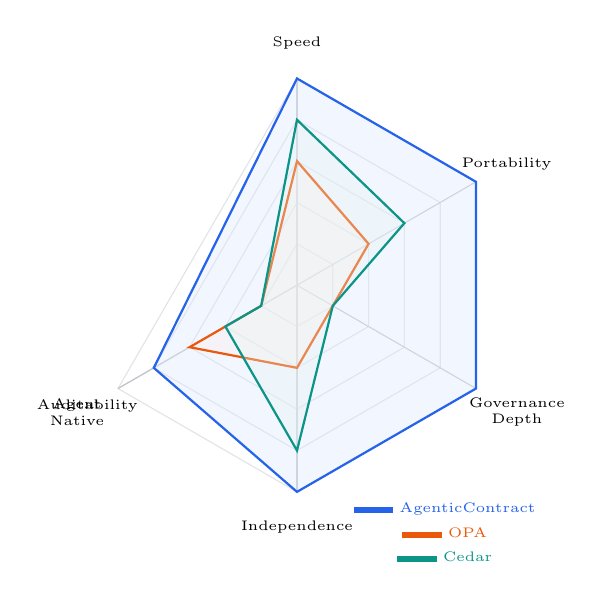
\begin{tikzpicture}[scale=0.75]
  % Axes at 60-degree intervals starting from top (90 degrees)
  % Axis 1: Speed (90), 2: Portability (30), 3: Governance Depth (-30)
  % Axis 4: Independence (-90), 5: Auditability (-150), 6: Agent Native (-210)

  % Grid rings (r=1..5, radius = r*0.7)
  \foreach \r in {1,2,3,4,5} {
    \draw[acgray!20, thin]
      (90:\r*0.7) -- (30:\r*0.7) -- (-30:\r*0.7) --
      (-90:\r*0.7) -- (-150:\r*0.7) -- (210:\r*0.7) -- cycle;
  }

  % Axis lines
  \draw[acgray!40, thin] (0,0) -- (90:3.5);
  \draw[acgray!40, thin] (0,0) -- (30:3.5);
  \draw[acgray!40, thin] (0,0) -- (-30:3.5);
  \draw[acgray!40, thin] (0,0) -- (-90:3.5);
  \draw[acgray!40, thin] (0,0) -- (-150:3.5);
  \draw[acgray!40, thin] (0,0) -- (210:3.5);

  % Axis labels
  \node[font=\tiny, align=center] at (90:4.1) {Speed};
  \node[font=\tiny, align=center] at (30:4.1) {Portability};
  \node[font=\tiny, align=center] at (-30:4.3) {Governance\\Depth};
  \node[font=\tiny, align=center] at (-90:4.1) {Independence};
  \node[font=\tiny, align=center] at (-150:4.1) {Auditability};
  \node[font=\tiny, align=center] at (210:4.3) {Agent\\Native};

  % AgenticContract (5,5,5,5,4,4)
  \draw[acblue, thick, fill=acblue!15, fill opacity=0.4]
    (90:3.5) -- (30:3.5) -- (-30:3.5) -- (-90:3.5) -- (-150:2.8) -- (210:2.8) -- cycle;

  % OPA (3,2,1,2,3,1)
  \draw[acorange, thick, fill=acorange!10, fill opacity=0.3]
    (90:2.1) -- (30:1.4) -- (-30:0.7) -- (-90:1.4) -- (-150:2.1) -- (210:0.7) -- cycle;

  % Cedar (4,3,1,4,2,1)
  \draw[acteal, thick, fill=acteal!10, fill opacity=0.3]
    (90:2.8) -- (30:2.1) -- (-30:0.7) -- (-90:2.8) -- (-150:1.4) -- (210:0.7) -- cycle;

  % Legend
  \node[font=\tiny, acblue] at (2.5, -3.8) {\rule{0.5cm}{2pt} AgenticContract};
  \node[font=\tiny, acorange] at (2.5, -4.2) {\rule{0.5cm}{2pt} OPA};
  \node[font=\tiny, acteal] at (2.5, -4.6) {\rule{0.5cm}{2pt} Cedar};
\end{tikzpicture}
\caption{Radar comparison across six dimensions. AgenticContract scores highest overall due to its purpose-built design for agent governance, though auditability is limited by single-writer constraints and agent-native integration relies on text-matching rather than a full policy language. OPA and Cedar excel at authorization expressiveness but lack governance depth (risk limits, obligations, violations) and agent-native integration.}
\label{fig:radar}
\end{figure}

Figure~\ref{fig:radar} compares AgenticContract against OPA and Cedar across six dimensions. The key differentiator is \emph{governance depth}: while OPA and Cedar provide binary allow/deny decisions, AgenticContract provides six distinct governance primitives, each with its own lifecycle and audit trail.

\subsection{Capacity Projections}

\begin{table}[t]
\caption{Real-world capacity projections for the \texttt{.acon} format. At typical agent governance scales (10--100 policies), file size remains under 100\,KB, supporting years of governance history in a single file.}
\label{tab:capacity}
\centering
\scriptsize
\setlength{\tabcolsep}{4pt}
\begin{tabular}{@{}lrrrr@{}}
\toprule
\textbf{Use Case} & \textbf{Entities} & \textbf{Size} & \textbf{Load} & \textbf{Yr/GB} \\
\midrule
Single agent & 10--50 & $<$25\,KB & $<$50\,\textmu{}s & 40K+ \\
Team (5 agents) & 50--200 & $<$100\,KB & $<$100\,\textmu{}s & 10K+ \\
Enterprise & 200--1K & $<$500\,KB & $<$1\,ms & 2K+ \\
Platform & 1K--10K & $<$5\,MB & $<$10\,ms & 200+ \\
\bottomrule
\end{tabular}
\end{table}

\subsection{Validation}

The implementation is validated by 288 tests across 8 suites, including stress tests at 1{,}000 policies, 500 risk limits, and 1{,}000 violations. Edge case coverage includes Unicode policy labels (Chinese, French, emoji), boundary values (\texttt{f64::MAX} risk limits, empty strings), exhaustive enumeration of all policy scopes and violation severities, and roundtrip file serialization at 200+ entities with BLAKE3 integrity verification. All tests pass with zero warnings on Rust 1.75+.

% ============================================================================
% 5. DISCUSSION
% ============================================================================
\section{Discussion}
\label{sec:discussion}

\textbf{Design trade-offs in the binary envelope.} The \texttt{.acon} format stores entity data as JSON within a binary header, trading storage density for schema flexibility. Adding new fields to policies or risk limits requires no format migration, no version negotiation, and no backward-compatibility code. The BLAKE3 checksum ensures integrity regardless of payload format. This follows the principle of making the common case fast (policy evaluation operates on deserialized in-memory structures at nanosecond speed) while making the rare case possible (schema evolution requires no migration tooling). The trade-off cost is approximately 2$\times$ storage overhead compared to a packed binary format---negligible at governance-typical scales of 10--500 entities.

\textbf{Graduated enforcement over binary allow/deny.} Four policy actions (Allow, Deny, RequireApproval, AuditOnly) provide richer semantics than the binary allow/deny model used by OPA and Cedar. An agent encountering RequireApproval can initiate the approval workflow; AuditOnly allows the action but creates an audit record. This graduated model enables a practical migration path: start with AuditOnly to observe agent behavior, escalate to RequireApproval for high-stakes actions, and apply Deny only after patterns are well understood. The append-only violation store complements this model by creating an immutable forensic record---an operator who wants to ``resolve'' a violation must create a new policy or obligation rather than erasing history.

\textbf{The expressiveness gap.} AgenticContract deliberately uses case-insensitive substring matching rather than a policy language. This avoids the complexity of language parsing, compilation, and optimization that OPA's Rego and Cedar require, at the cost of lower expressiveness. Complex conditional logic (``allow if user is admin AND resource is in department X AND time is business hours'') requires multiple cooperating policies rather than a single expression. For agent governance, where policies are typically 10--100 human-readable rules, this trade-off favors simplicity. However, as agent deployments mature, richer policy languages may become necessary, and the engine's modular evaluation path is designed to accommodate alternative matchers.

\textbf{Limitations.} The engine does not implement file locking; concurrent writes from multiple processes may corrupt the \texttt{.acon} file, restricting deployment to single-writer, multiple-reader configurations. Policy evaluation is $O(n)$ in the number of active policies---at 1{,}000 policies (72.8\,\textmu{}s) this remains negligible, but workloads exceeding 10{,}000 policies would require index-based evaluation (trie or hash map on scope). The system is designed for local-first, single-file governance; multi-node coordination requires external consensus protocols. Near-term priorities include sidecar file locking (following the pattern from AgenticMemory~\cite{agenticmemory2026}), policy indexing for large workloads, and a WASM build for browser-based governance.

% ============================================================================
% 6. CONCLUSION
% ============================================================================
\section{Conclusion}
\label{sec:conclusion}

This paper presented AgenticContract, a self-contained policy engine that models six governance primitives---policies, risk limits, approvals, conditions, obligations, and violations---in a single binary file format with BLAKE3 integrity verification. The key contribution is demonstrating that runtime policy enforcement for autonomous AI agents can be achieved with sub-microsecond latency and zero external dependencies, removing the tension between governance rigor and operational speed.

Criterion benchmarks confirm 49.3\,ns single-policy evaluation, 72.8\,\textmu{}s for 1{,}000-policy workloads, 43.9\,ns risk limit checks, and sub-millisecond file I/O for 100 entities---performance that is invisible relative to LLM inference costs of 10--50\,ms per token. The system is implemented in 7{,}382 lines of Rust across four crates, validated by 288 tests across 8 suites, and integrated via the Model Context Protocol for zero-configuration agent adoption.

The graduated enforcement model (Allow, Deny, RequireApproval, AuditOnly) with append-only violation forensics provides richer governance semantics than existing policy engines, which model only binary allow/deny decisions. As AI agents gain autonomy in production environments, the gap between alignment training and runtime enforcement will widen. AgenticContract addresses this gap by treating governance not as a constraint on agent capability, but as a structured, auditable, and computationally negligible layer that enables agents to operate with both autonomy and accountability.

AgenticContract is available as an open-source MIT-licensed project at \url{https://github.com/agentralabs/agentic-contract}.

\bibliographystyle{plain}
\bibliography{agenticcontract-references}

\end{document}
